\subsection*{Overview}
Within the retrain.py script \parencite{retrainInception}, as mentioned in
previous experiments, there are various parameters that can be set and changed.
Various combinations of these parameters were changed to see if it would increase the
test accuracy of the model.

\subsection*{Network Architecture}
The Inception V3 architecture was used for this model.

\subsection*{Dataset}
The Food-101 dataset \parencite{food101} with additional classes, as per
\ref{inception}, was used for this model.

\subsection*{Libraries}
The libraries in use for this experiment are tensorflow and numpy.

\subsection*{Script}
Script as seen in \ref{inception} but with some additions to calculate Top 5 accuracy as seen
below:

\begin{lstlisting}
python retrain_top5.py \ --image_dir
~/dataset_directory \ --how_many_training_steps 4000 \ --learning_rate 0.01 \
--testing_percentage 10 \ --validation_percentage 10
\end{lstlisting}

Top 5 accuracy of the model was als calcultaed using the code below.
\begin{lstlisting}[style=Python]
print('Top 5 Evaluation')
#Variables used to store a list of all classes, the amount of images tested,
# the amount of images with a top 5 accuracy and the sum of the highest probabilities
classes = list(image_lists.keys())
image_count = 0
top_5_count=0
total_of_top1_probs = 0
i = 0 
class_counter = 0

#Loops through all test images, selecting 10 images per class 
#and running them through the method in 'label_image.py'.
while(i < len(test_bottlenecks)):
  class_counter += 1
  
  if class_counter > 10:
    i = int(round((i + len(test_bottlenecks)/len(classes)) - 10))
    class_counter = 0
  else:
    image_count += 1
    results_from_classifier = label_image.runModel(test_filenames[i])
    results = results_from_classifier[0]
    probabilities = results_from_classifier[1]

    if classes[test_ground_truth[i]] in results:
      top_5_count += 1
    else:
      print("Expected:  " + classes[test_ground_truth[i]])
      for result in results:
        print("Classes: " + result)
      print("")

    total_of_top1_probs += max(probabilities)
    i = i + 1
print(str(top_5_count))
average_probabilities = total_of_top1_probs/(len(classes*10))

#Prints out the amount of test images used, the top 5 accuracy
# and the average probability of predictions.
print("Amount of test images: " + str(image_count))
print("Top 5 Accuracy: " + str((top_5_count/image_count)*100))
print("Average probability: " + str(average_probabilities))
\end{lstlisting}

Method from label\_image.py.
\begin{lstlisting}[style=Python]
def runModel(file_name):
  model_file = \
    "/tmp/output_graph.pb"
  label_file = "/tmp/output_labels.txt"
  input_height = 299
  input_width = 299
  input_mean = 128
  input_std = 128
  input_layer = "Mul"
  output_layer = "final_result"

  graph = load_graph(model_file)
  t = read_tensor_from_image_file(file_name,
                                  input_height=input_height,
                                  input_width=input_width,
                                  input_mean=input_mean,
                                  input_std=input_std)

  input_name = "import/" + input_layer
  output_name = "import/" + output_layer
  input_operation = graph.get_operation_by_name(input_name)
  output_operation = graph.get_operation_by_name(output_name)

  with tf.Session(graph=graph) as sess:
    results = sess.run(output_operation.outputs[0],
                      {input_operation.outputs[0]: t})
  results = np.squeeze(results)

  top_k = results.argsort()[-5:][::-1]
  labels = load_labels(label_file)
  
  setIndex = False

  top5_results = [None] * 5
  index = 0
  for i in top_k:
    top5_results[index] = labels[i]
    index += 1

  final_results = [top5_results, results]
  return final_results
\end{lstlisting}

Some further parameters could be set such as:
\begin{itemize}
	\item{--flip\_left\_right}
	\item{--random\_crop}
	\item{--random\_scale}
	\item{--random\_brightness}
\end{itemize}

\begin{figure}
    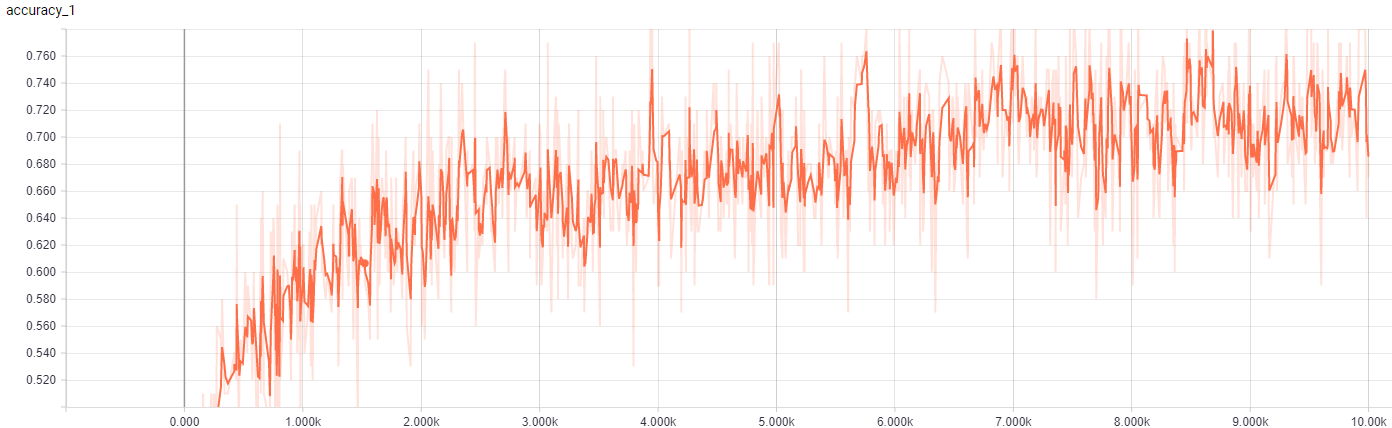
\includegraphics[scale=0.5]{model_test}
     \caption{Graph of accuracy of the test dataset during training}
     \label{fig:model_train_test}
\end{figure}

\begin{figure}
    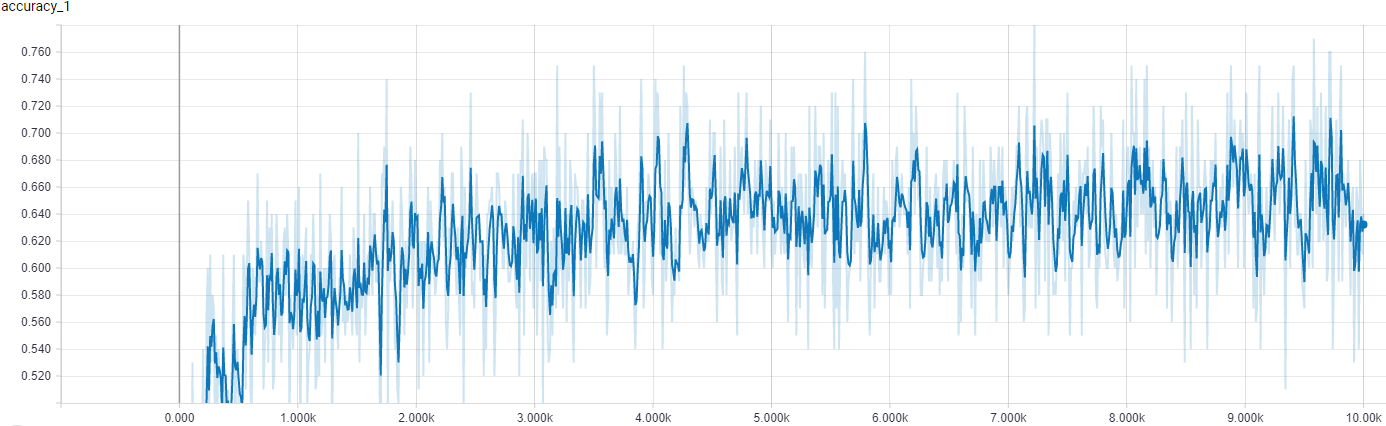
\includegraphics[scale=0.5]{model_val}
     \caption{Graph of accuracy of the validation dataset during training}
     \label{fig:model_train_val}
\end{figure}

\begin{figure}
    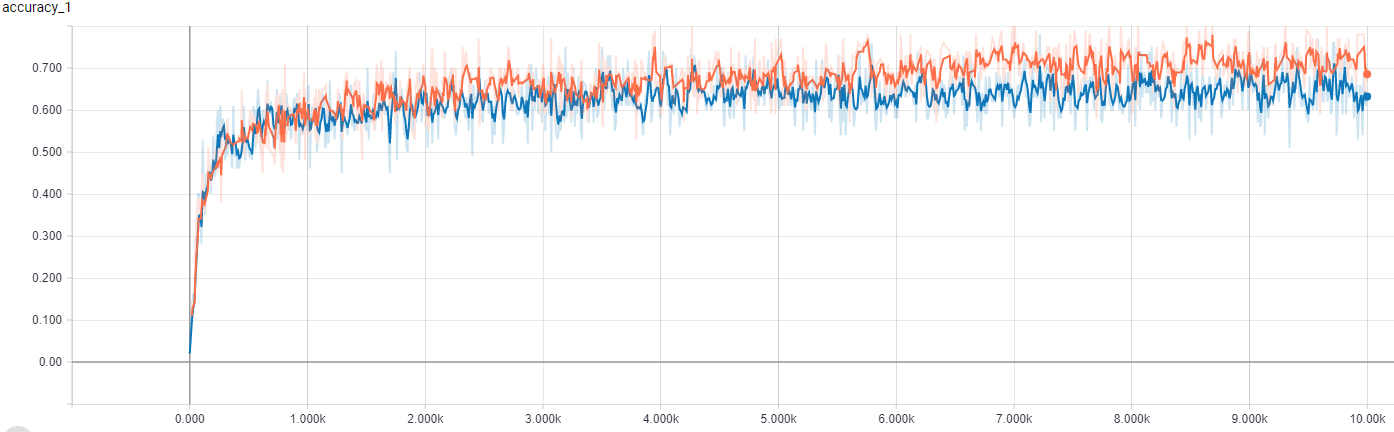
\includegraphics[scale=0.4]{test_val_accuracy}
     \caption{Comparison of accuracy}
     \label{fig:test_val_accuracy}
\end{figure}

\begin{figure}
    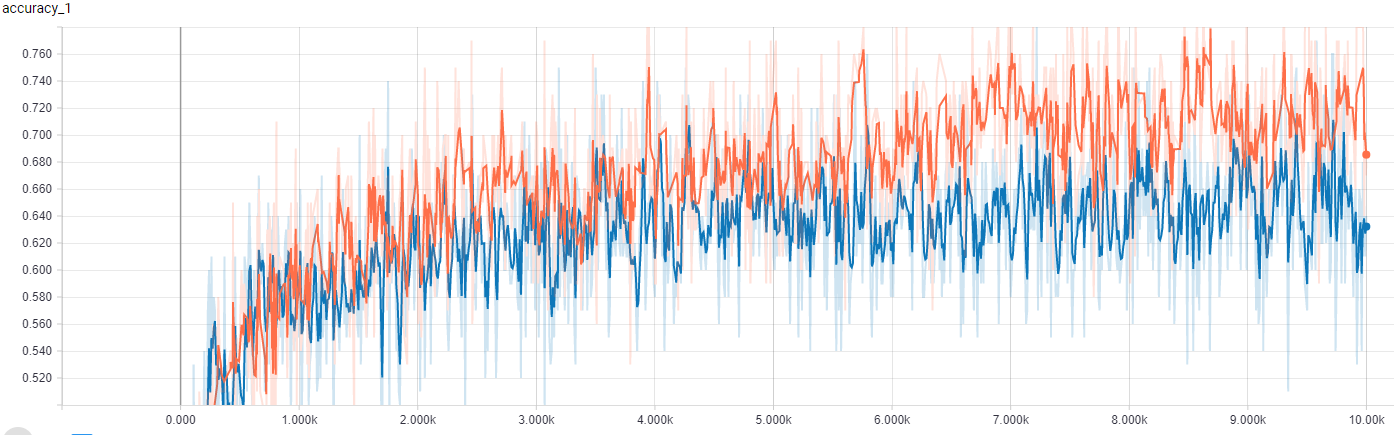
\includegraphics[scale=0.4]{test_val_accuracy_refined}
     \caption{Comparison of accuracy}
     \label{fig:test_val_accuracy_refined}
\end{figure}


\begin{table}[]
	\centering
	\caption{Comparison of parameters}
	\label{parameter_tuning_table}
	\begin{tabular}{|l|l|l|l|l|l|}
  \hline
		\textbf{Parameter Tuning} & \textbf{Steps} & \textbf{Learning Rate} & \textbf{Test} \% & \textbf{Validation} \% &
		\textbf{Results} \\ \hline
		Configuration 1  & 8,000  & 0.01       & 10 & 10       &
		59.1\%  \\ \hline
		Configuration 2  & 8,000  & 0.10           & 10 & 10       &
		65.8\%  \\ \hline
		Configuration 3  & 10,000 & 0.10           & 10 & 10       &
		66.3\%  \\ \hline
		Configuration 4  & 12,000 & 0.10           & 10 & 10       &
		66.6\%  \\ \hline
		Configuration 5  & 10,000 & 0.20           & 10 & 10       &
		66.0\%  \\ \hline
		Configuration 6  & 10,000 & 0.10           & 15      & 15            &
		66.3\%  \\ \hline
	\end{tabular}
\end{table}

\subsection*{Results}
The results of each set of parameters can be seen in Table
\ref{parameter_tuning_table}.
Using the parameters of 10,000 steps, and a learning rate of 0.1 and therefore a final test accuracy of 66.3\%, the model achieved a Top 5 accuracy of 85.96\%.
This figure was calculated from 1090 images in the test dataset and the average probability of the predictions were at 0.62.


\subsection*{Empirical Analysis}
The set of parameters that seem to be the most
effective are 10000 steps with a 0.1 learning rate. Graphs of this model can be
see in Figures \ref{fig:model_train_val} and \ref{fig:model_train_test}. These
are based on the validation set and then the test set respectively. A side by
side comparison can also be seen in Figures \ref{fig:test_val_accuracy} and
\ref{fig:test_val_accuracy_refined} where orange is for during training and blue
for the validation set.

There were two separate factors that each increased classification accuracy of
about 5\% each. These were training steps and learning rate.

Training steps are related to the number of images so before, when the training
steps were at 4000, not all of our training images were being used. As the steps were increased
twofold we saw a 3.8\% increase in accuracy.

Another parameter that increased accuracy significantly was learning rate. The
default learning rate is 0.01 which was increased to 0.1. This resulted in an
increase of 6.7\%. This is most likely due to the fact that since we are only
looking at the last layer, we can afford to change the weights more
significantly.

The Top 5 accuracy of the model was quite good but it was not run on the same number of images as the final test accuracy. This is due to the fact that tensorflow does not have an API for calculating Top 5 accuracy. As a result, it had to be calculated manually and this is very time intensive. The average probability of 0.62 is interestingly close to the overall Top 1 accuracy.
